\documentclass[usenames,dvipsnames,tikz]{standalone}
\usepackage{xcolor}
\colorlet{tBlue}{RoyalBlue!35!Cerulean}
\colorlet{tRed}{Red}
\usepackage{tikz}
\usepackage{standalone}
\begin{document}
	
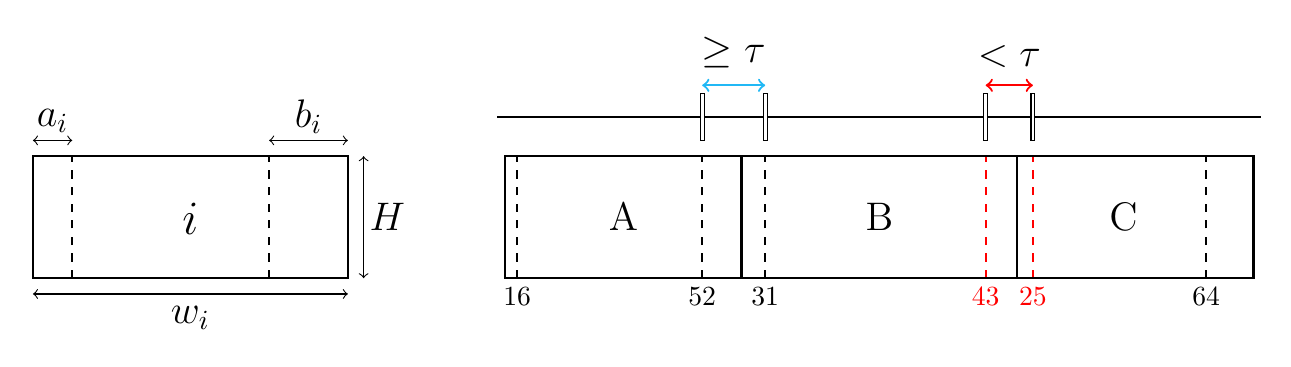
\begin{tikzpicture}
%\draw [help lines] (-1,-2) grid (17,5);

% item i
\draw [thick] (0,0) rectangle (4,1.55);
\draw [thick, dashed] (0.5,0) -- (0.5, 1.55);
\draw [thick, dashed] (3,0) -- (3, 1.55);
\node at (2,0.75) {\LARGE{$i$}};

%arrow and label for width w_i
\draw [<->] (0,-.2) -- (4,-.2);
\node at (2, -.5) {\Large{$w_i$}};

%arrow and label for score width a_i
\draw [<->] (0, 1.75) -- (0.5, 1.75);
\node at (0.25, 2) {\Large{$a_i$}};

%arrow and label for score width b_i
\draw [<->] (3, 1.75) -- (4, 1.75);
\node at (3.5, 2.05) {\Large{$b_i$}};

%arrow and label for height H
\draw [<->] (4.2,0) -- (4.2,1.55);
\node at (4.5,0.775) {\Large{$H$}};

%-----------------
%red line first so that they appear under black lines
\draw [thick, tRed, dashed] (12.1,0) -- (12.1,1.55); %4
\draw [thick, tRed, dashed] (12.7,0) -- (12.7,1.55); %2

%3 items ordered
\draw [thick] (6,0) rectangle (15.5,1.55);
%between items A and B
\draw [thick] (9,0) -- (9,1.55);
%between items B and C
\draw [thick] (12.5, 0) -- (12.5,1.55);

%labels for items A, B and C
\node at (7.5,0.775) {\Large{A}};
\node at (10.75,0.775) {\Large{B}};
\node at (13.85,0.775) {\Large{C}};

%score lines and score width labels for item A
\draw [thick, dashed] (6.15,0) -- (6.15,1.55); %1
\draw [thick, dashed] (8.5,0) -- (8.5,1.55); %5
%\node [below] at (7.075,0) {1};
%\node [below] at (9.75,0) {5};
\node [below] at (6.15,0) {16};
\node [below] at (8.5,0) {52};

%score lines and score width labels for item B
\draw [thick, dashed] (9.3,0) -- (9.3,1.55); %3
%\draw [thick, red, dashed] (13.1,0) -- (12.1,1.55); %4 moved to top
%\node [below] at (10.15,0) {3};
%\node [below] at (13.3,0) {\textcolor{tRed}{4}};
\node [below] at (9.3,0) {31};
\node [below] at (12.1,0) {\textcolor{tRed}{43}};

%score lines and score width labels for item C
%\draw [thick, red, dashed] (13.7,0) -- (12.7,1.55); %2 moved to top
\draw [thick, dashed] (14.9,0) -- (14.9,1.55); %6
%\node [below] at (13.6,0) {\textcolor{tRed}{2}};
%\node [below] at (16.2,0) {6};
\node [below] at (12.7,0) {\textcolor{tRed}{25}};
\node [below] at (14.9,0) {64};

%------------------

%Bar with knives 
\draw [thick] (5.9,2.05) -- (15.6,2.05);

%knives for items A and B
\filldraw[fill=white, draw=black, thin] (8.475,1.75) rectangle (8.525,2.35);
\filldraw[fill=white, draw=black, thin] (9.275,1.75) rectangle (9.325,2.35);
%\draw [thick] (9.5,1.75) -- (9.5,2.35);
%\draw [thick] (10.3,1.75) -- (10.3,2.35);

%knives for items B and C
\filldraw[fill=white, draw=black, thin] (12.075,1.75) rectangle (12.125,2.35);
\filldraw[fill=white, draw=black, thin] (12.675,1.75) rectangle (12.725,2.35);
%\draw [thick] (13.1,1.75) -- (13.1,2.35);
%\draw [thick] (13.7,1.75) -- (13.7,2.35);


%constraint label for score widths between items A and B (feasible, >= tau)
\draw [thick, <->, tBlue] (8.5, 2.45) -- (9.3, 2.45);
\node [above] at (8.9,2.55) {\Large{$\geq \tau$}};

%constraint label for score widths between items B and C (infeasible, < tau)
\draw [thick, <->, tRed] (12.1, 2.45) -- (12.7, 2.45);
\node [above] at (12.4,2.55) {\Large{$< \tau$}};

%\draw [<->] (3.5,2.2) -- (4.5,2.2);
%\node at (4, -.4) {\scriptsize $\geq \tau$};

\end{tikzpicture}
	
\end{document}